\documentclass[12pt]{ctexart}

\usepackage[hmargin=3.18cm,vmargin=2.54cm]{geometry}
\usepackage{graphicx}
\usepackage{tabularx}
\usepackage{multicol}
\usepackage{float}
\usepackage{amsmath}
\usepackage{enumitem} 
\usepackage{subfigure}

% 重定义有序列表样式
\renewcommand{\labelenumi}{(\arabic{enumi})}

\ctexset{
  % 修改 part 标题样式
  part={
      format=\heiti\centering\zihao{3}
  },
  % 修改 section 标题样式
  section={   
    % 分隔符为 、
    name={,、},
    % 设置 section 标题为黑体、右对齐、小三号字
    format=\heiti\raggedright\zihao{-3}\bfseries,
    % 中文编号
    number={\chinese{section}},
    % 编号与标题名的间距
    aftername=\hspace{0.2em}
  },
  subsection={   
    % 无分隔符
    name={},
    % 设置 section 标题为宋体、右对齐、四号字
    format=\songti\raggedright\zihao{4}\bfseries,
    % 编号与标题名的间距
    aftername=\hspace{0.8em}
  },
  subsubsection={   
    name={},
    % 设置 section 标题为宋体、右对齐、小四号字
    format=\songti\raggedright\zihao{-4}\bfseries,
    % 编号与标题名的间距
    aftername=\hspace{0.8em}
  },
}

\begin{document}

\pagestyle{plain}

\thispagestyle{empty}
\part*{单相在线式不间断电源}

\noindent{\textbf{摘要:}
  本系统由输入整流升压电路级联PWM全桥逆变电路构成。前级直流部分采用 Boost 升压电路,交流部分采用不控整流后接 Boost 升压电路。后级PWM全桥逆变电路产生稳定可控的正弦波。控制器采用电压闭环分别控制直流母线电压及交流输出电压,检测到断开交流电源后,可即时切换至直流电源供电。该电路输出电压稳定,交流供电时负载调整率和电压调整率小于0.1\%,频率稳定在50Hz,误差小于0.02\%。直流供电额定状态下系统效率可达到96.1\%。该不间断电源输出电压为正弦波,THD小于2\%。
}

\noindent{\textbf{关键词:}
  不控整流\hspace{0.5em}
  Boost电路\hspace{0.5em}
  PWM全桥逆变\hspace{0.5em}
  电压控制\hspace{0.5em}
}
\newpage

\setcounter{page}{2}

\section{方案论证}
\subsection{比较与选择}
\subsubsection{交流回路拓扑选择}
方案一:不控整流级联Boost电路。不控整流电路结构简单,响应迅速,输出稳定,方便整体电路的控制。

方案二:PWM整流器级联Boost PFC电路。PWM整流器无整流二极管,功耗较低。但Boost PFC电路拓扑结构与控制系统较为复杂,会增加不必要的控制系统复杂度。

综合考虑,为了使控制更加稳定并简化整体电路,选择方案一。

\subsubsection{电压控制方案选择}
方案一:直接对逆变器的输出电压进行采集并进行控制,中间电路无需设置测量模块。这种方式结构简单,但是对控制系统的要求较高,难以保证控制稳定性及精度。

方案二:将Boost输出母线电压及逆变输出电压分开采集和控制,电路耦合程度更低,控制精度更高,响应时间更短,使得最终输出的电压更加稳定。

综合考虑,为了保证更高的电压控制精度和更好的稳定性,选择方案二。

\subsubsection{系统总体方案描述}
系统包括不控整流电路、Boost电路、逆变器电路、交流电压电流测量电路、直流电压测量电路以及单片机控制电路和保护电路,如图\ref{system_block_diagram}所示。

\begin{figure}[htbp!]
  \centering
  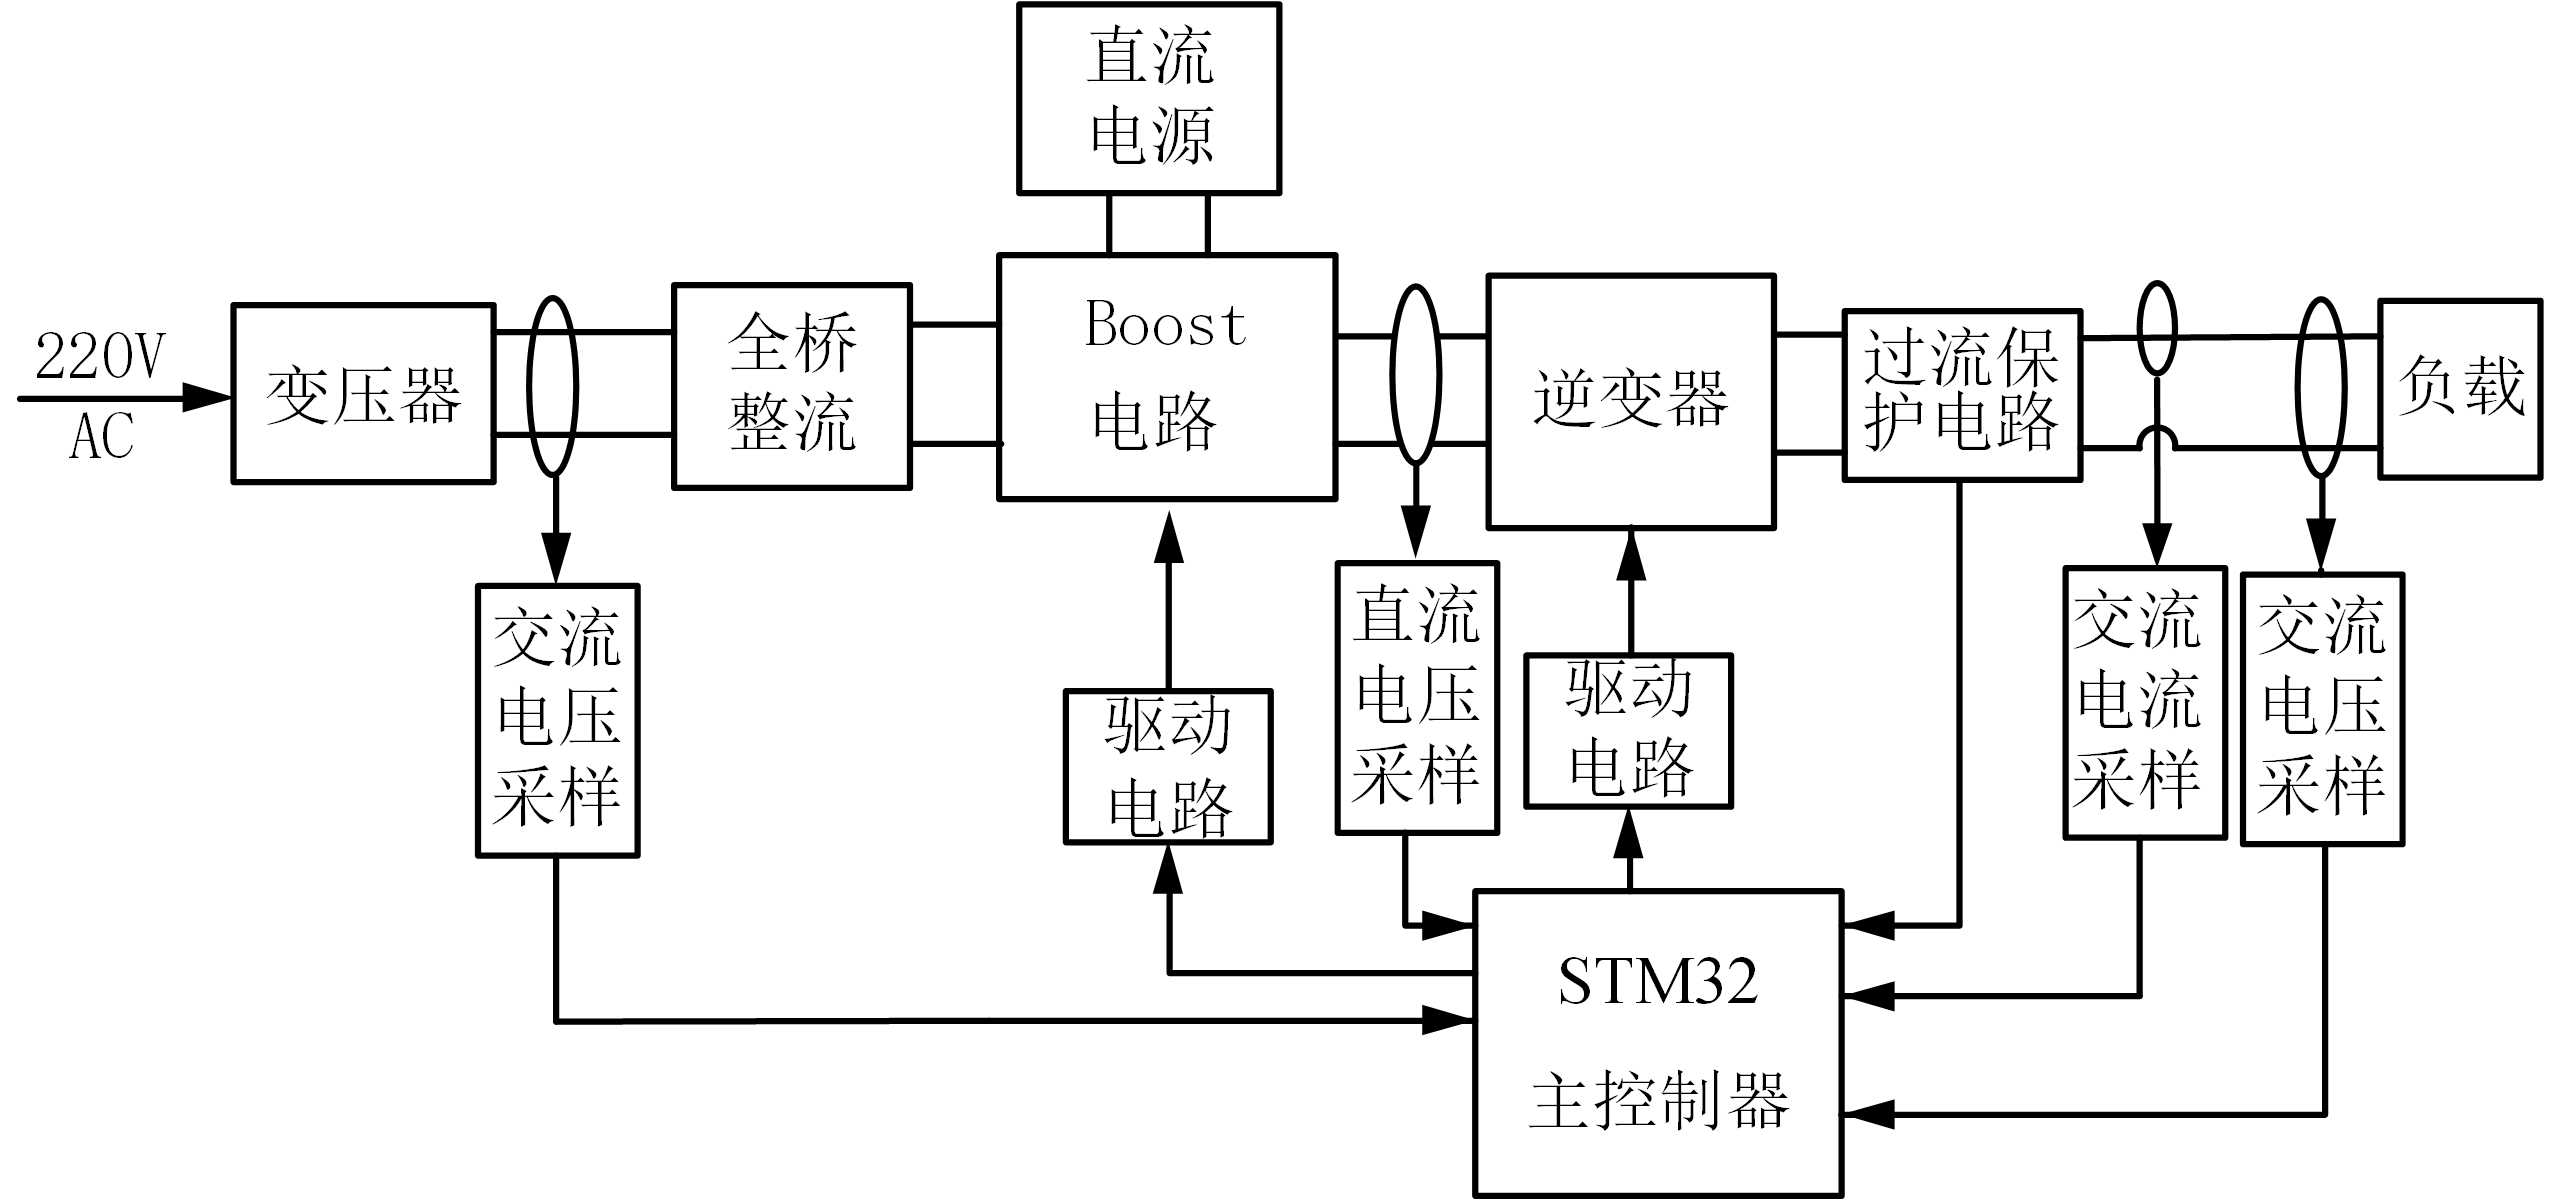
\includegraphics[width=0.9\linewidth]{img/system block.png}
  \caption{系统总框图}
  \label{system_block_diagram}
\end{figure}

\section{理论分析与计算}
\subsection{提高效率的方法}
系统的损耗主要包括开关管的开关损耗、导通损耗和电感铜耗、铁耗、电容等效电阻等无源器件的损耗。因此提高效率应尽可能减小这些因素的损耗。

\begin{enumerate}[leftmargin=0pt,itemindent=!]
  \item 减小开关管开关损耗的方法
 
  \qquad 选择合适的开关频率:过高的开关频率会增大开关管的损耗,但开关频率过低则会增大滤波电感的体积和重量。综合考虑,开关频率取20kHz。

  \qquad 选择合适的开关管:开关管会有开关损耗,结电容和电路分布电感影响其开关损耗。因此开关管的反向恢复电容尽量小。

  \item 减小开关管导通损耗的方法
  
  \qquad 选择合适的开关管:开关管的导通电阻影响其导通损耗,因此开关管导通电阻越小越好。但开关管的寄生电容和导通电阻参数矛盾,二者往往不能同时最小,需折衷考虑。

  \item 减小无源器件损耗的方法
  
  \qquad 选择合适的电感:电感太小,电流谐波抑制能力差;电感太大,铜耗大。因此需选择大小合适的电感。同时,电感设计时应适当降低电流密度和磁通密度,减小损耗。选择电容时应采用并联多个小电容等方法,使等效串联电阻尽量小。
\end{enumerate}

\subsection{Boost电路输出稳压控制方法}
在Boost电路闭环控制中,采样输出直流电压实时值,与参考设定值 求差,再送入PI控制器进行计算,将计算值输入PWM控制器调控PWM波对应的占空比,通过变换器输出调控后的直流电压。控制框图如图\ref{dc_control}所示。

\begin{figure}[htbp]
  \centering
  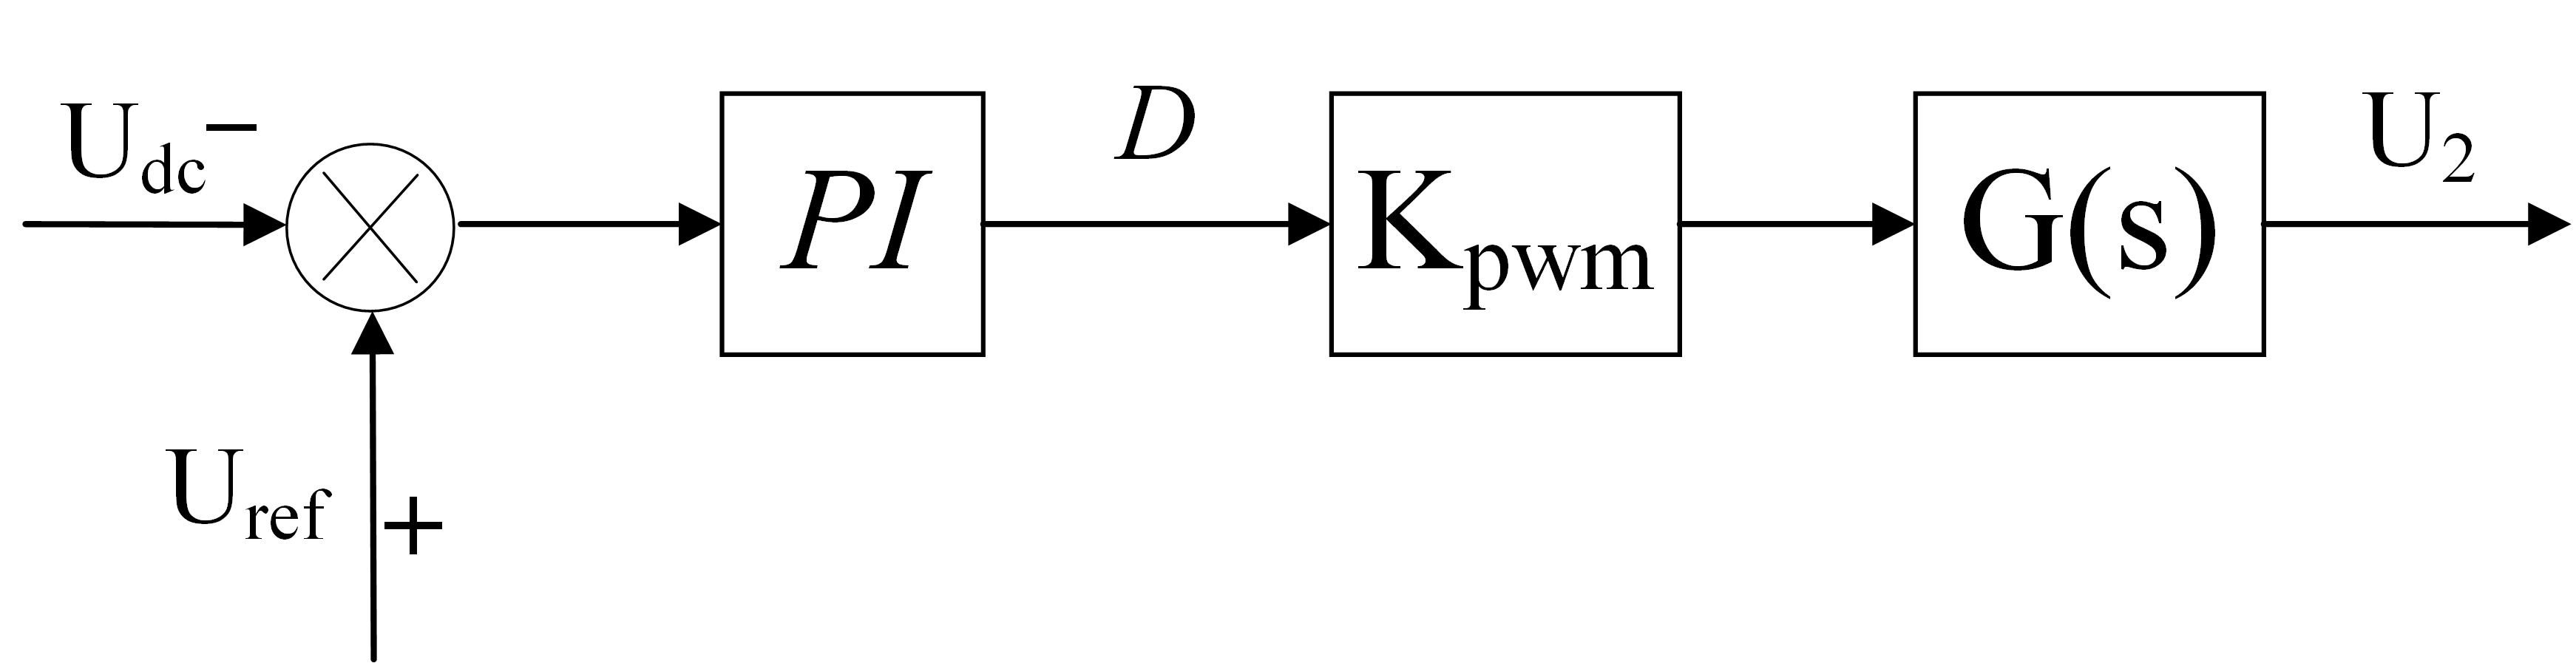
\includegraphics[width=0.9\linewidth]{img/dc control.png}
  \caption{直流电压控制策略框图}
  \label{dc_control}
\end{figure}



\end{document}

% 你可能会用到……

% 多张图并排

% \begin{figure}[htbp]
%   \begin{minipage}[t]{0.5\linewidth}
%     \centering
%     \includegraphics[width=0.9\linewidth]{img/figure_1.png}
%     \label{label_1}
%     \caption{figure 1}
%   \end{minipage}
%   \begin{minipage}[t]{0.5\linewidth}
%     \centering
%     \includegraphics[width=0.9\linewidth]{img/figure_2.png}
%     \label{label_2}
%     \caption{figure 2}
%   \end{minipage}
% \end{figure}

% 如果你使用的是 VSCode,你可以把这些内容添加到 snippets

% 	"default_image": {
% 		"prefix": "image",
% 		"body": [
% 			"\\begin{figure}[htbp]",
%   		"  \\centering",
%   		"  \\includegraphics[width=${0:0.9\\linewidth}]{img/$1}",
%   		"  \\label{$2}",
%   		"  \\caption{$3}",
% 			"\\end{figure}"
% 		],
% 		"description": "Insert a plain image"
% 	}